\section{Introduction}
Various areas, including social networks, chemical compounds, graph neural networks, and citation networks, use graphs as their underlying data structure. With the widespread adoption of graphs and the increasing graph size, many algorithms have been proposed to analyze graphs efficiently. Among these algorithms, subgraph matching has always played an essential role in graph data mining.

The goal of subgraph matching is to find all subgraphs in a data graph $G$ that are isomorphic to a given query graph $q$. Though the problem is NP-complete, many approaches  \cite{bhattarai2019ceci,guo2020gpu,tran2015fast,shi2020graphpi,bi2016efficient,zeng2020gsi,sun2020subgraph,guo2020exploiting,sun2020rapidmatch,lin2016network} have been proposed to speed up subgraph matching in recent years. All these approaches adopt a similar 3-step procedure. They first build candidate sets and auxiliary data for query vertices, then generate a matching order for query vertices based on candidate sets and auxiliary data and finally match $q$ in $G$ according to the matching order. Most previous works mainly focus on generating an effective matching order that can reduce the number of intermediate results during subgraph matching. For example, the main idea of the matching order generation algorithm proposed in \cite{bi2016efficient} is to match all non-tree edges regarding any spanning tree of $q$ as soon as possible to eliminate invalid subgraph candidates in the early stages of the matching process. We borrow this idea when designing our matching order generation algorithm.

Some works \cite{lin2016network,guo2020gpu,tran2015fast,zeng2020gsi,guo2020exploiting} focus on optimizing subgraph matching on GPUs, and GSI \cite{zeng2020gsi} achieves the best performance among all these approaches. GSI designs an edge label partitioned CSR (PCSR) format for a data graph to speed up accessing vertex neighbors. To build a PCSR format for a data graph, GSI first groups edges and corresponding vertices by the edge label into edge label partitions. Then, GSI builds a GPU-based CSR format for each edge label partition, which is the PCSR format. In order to find the position of a given vertex ID (VID) in PCSR, GSI adopts a hash function to map VIDs to positions (hash-PCSR), which needs many empty entries to reduce collisions (GSI uses 30 empty entries for each VID). In our approach, we also utilize PCSR format but replace the hash function with interval indexes (interval-PCSR). Additionally, we design a VID mapping algorithm for vertices in $G$ to map old VIDs to new VIDs, which can create more contiguous VIDs in each edge label partition and hence reduce the number of intervals. GSI proposes a Prealloc-Combine approach to make the parallel write of intermediate results more efficient. Nevertheless, this approach needs to launch two extra GPU kernels to write intermediate results to the right place. Unlike GSI, we utilize atomic operations inside the GPU kernel to calculate right positions for intermediate results. Therefore, we do not need extra GPU kernels.

All the abovementioned works match vertices of $q$ one by one, and thus need to write the intermediate results after extending one vertex and read the same intermediate results before extending the next vertex. The write and read operations are time-consuming, especially when the size of intermediate results is significant. To mitigate the cost of write and read operations, Lai et al. \cite{lai2015scalable} utilize MapReduce to implement a double-edge extension method. \RV{Their approach iteratively matches the query graph by a TwinTwig that consists of one edge (extension pattern 0 in Figure \ref{fig:extpattern}) or two incident edges of a vertex (extension patterns 1 and 3 in Figure \ref{fig:extpattern})}. However, there are three inherent limitations in \cite{lai2015scalable}. First, edges in a TwinTwig must grow from the same vertex, which means their approach can not handle extension patterns 2, 4, and 5-7 in Figure \ref{fig:extpattern}. Second, a TwinTwig contains at most two edges, but more than two backward edges can be processed at the same time. \RV{Third, they use a simple method to generate results for extension pattern 1}, which causes a number of unnecessary memory accesses to neighbors.

To overcome limitations of \cite{lai2015scalable}, \RV{we propose the N-vertex extension method (NV-ext), which iteratively matches the query graph by as many vertices as possible}. First, our approach can extend vertices from different source vertices and thus can handle all extension patterns in Figure \ref{fig:extpattern}. Second, our approach can match as many edges as possible in a single GPU kernel (illustrated in Section \ref{sec:eliphase}). Third, we design an optimized algorithm (Algorithm \ref{algo:optDV}) to reduce unnecessary memory accesses for extension pattern 1. Moreover, we develop a new matching order generation algorithm (Algorithm \ref{algo:genmatchorder}) that is designed specifically for our NV-ext method.

 %A more aggressive method is triple-vertex extension. This method is applicable, but we do not implement it in this work. The reason is two-fold. First, in our NV-ext method, the register usage has exceeded the GPU hardware resource limit in some cases, which can significantly increase the memory access latency for some variables. Hence, it is fairly easy to speculate that the triple-vertex extension method will lead to more registers overflow than our approach. Second, the triple-vertex extension method needs a more complicated scheme to implement an efficient parallel write of intermediate results, which is not the focus of this work.

\begin{figure}
\centering
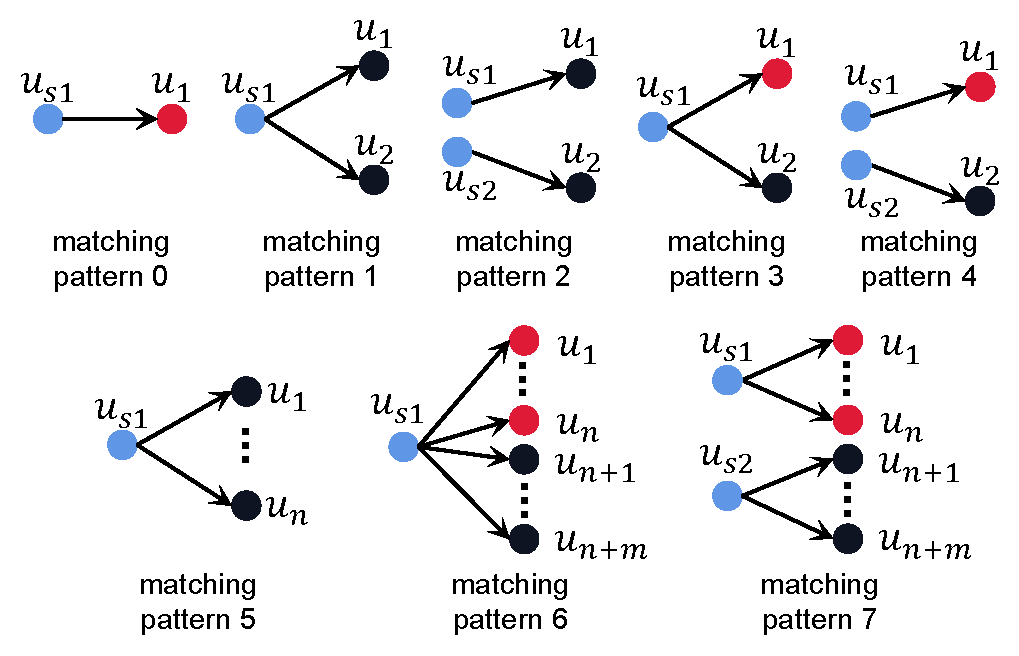
\includegraphics[width=0.9\columnwidth]{./figure/extpattern.eps}
\caption{\RV{Extension patterns supported by our N-vertex extension method. $u_{s1}$ and $u_{s2}$ represent matched query vertices, and can be any vertex labels. \{$u_1, \cdots, u_{n}$\} and 
\{$u_{n+1}, \cdots, u_{m}$\} represent query vertices to be matched, and vertices in the same set have the same vertex label. Edges in the the same extension pattern have the same edge label.}}	
\label{fig:extpattern}
\end{figure}

 We validate our approach from three aspects: (1) Experimental results show that our interval-PCSR significantly reduces the space cost and searching time of hash-PCSR by 83\% and 58\% respectively; (2) We obtain an average speedup of $5\times$ over GSI for subgraph matching; (3) Compared to the single-vertex extension method (SV-ext), which is modified based on our NV-ext method, our approach reduces the matching time by 15.9\% on average.

 To summarize, we make the following contributions:
 \begin{itemize}
  \item We propose an interval-PCSR format and a mapping algorithm that can generate more contiguous VIDs in each edge label partition. Our interval-PCSR significantly reduces the space cost and searching time of hash-PCSR of GSI.
  \item We propose a NV-ext method that can match as many query vertices as possible to reduce the number of read and write operations of intermediate results.
  \item We propose a new matching order generation algorithm and a new parallel write scheme to accommodate our NV-ext method.
\end{itemize}
